% ! TeX root = ../../main.tex
\chapter{Design e tecnologie}
\section{Requisiti}
% In  questo contesto il contributo di questa tesi mira ad aumentare l'interesse e la consapevolezza sul tema della ecosostenibilità e sul risparmio di carta attraverso l'integrazione di una applicazione per smartphone e un totem multimediale con anche l'aiuto della realtà aumentata e la \textit{gamification}.
Questa tesi ha l'obiettivo di sviluppare l'applicativo per un totem multimediale che si integri con l'applicazione mobile per smartphone BoschettoAR facente oarte del progetto ReMade.
Nello specifico devono essere presenti diverse schermate che mostrano i progressi del progetto ReMade e i dati condivisi degli utenti.
%
\subsection{Requisiti funzionali}
Più precisamente devono essere presenti le schermate Home, statistiche, Classifica e Informazioni.

La schermata principale chiamata \enquote{Home} deve mostrare un bosco ricco di alberi visto dall'alto (si vedono solo le chiome). Al tocco di un albero vengono mostrati i  (nickname,\dots) e le statistiche (contatori badge,...) relative all'utente corrispondente. Gli alberi devono cambiare la loro rappresentazione in base al livello raggiunto dall'utente.

La schermata delle Statistiche invece deve mostrare diversi contatori provvisti di un'icona rappresentativa, di una \textit{label} (etichetta) che specifica a cosa si riferisce il dato mostrato e infine il valore con unità di misura. Ciascun contatore al tocco deve mostrare una breve descrizione che spieghi il significato del valore.

La penultima pagina, quella della classifica, deve mostrare una classifica dei 10 migliori utenti sulla base della co2 risparmiata.
Gli elementi della classifica devono avere la posizione, il nickname dell'utente, la rappresentazione del livello dell'utente e quanta co2 hanno risparmiato.

La pagina delle Informazioni, deve mostrare diverse informazioni quali i calcoli fatti per ricavare i dati nella pagina delle statistiche e dettagli sul progetto a cui fa parte. Questa schermata deve essere il quanto più semplice possibile e può prevedere altre sezioni in caso di ulteriori informazioni da mostrare.

Oltre alle diverse pagine, deve essere presente una sezione o schermata sempre accessibile e visibile che permetta di avviare la modalità di caricamento dei dati utente dall'app al totem indistintamente dalla schermata visualizzata. Avviata la modalità deve essere visualizzato il qrcode identificativo del totem che verrà scansionato dall'app mobile.
%
\subsection{Requisiti non funzionali}
\begin{itemize}
    \item Il sistema deve essere scalabile in modo da permettere l'aggiunta di nuovi totem interattivi e gestire simultaneamente più richieste di condivisione dei dati dall'applicazione.
    \item L'interfaccia deve apparire familiare ed intuitiva fin dall'inizio, in modo da permettere un utilizzo immediato e non scoraggiare gli utenti all'interazione.
    \item La sincronizzazione dei dati deve essere, per quanto possibile, immediata in modo da mostrare sempre dati aggiornati.
\end{itemize}
%
%
%
\section{Design e mockup}
Prima di analizzare le scelte di \textit{design} e di mostrare i diversi \textit{mockup} sviluppati si introducono i significati delle due parole in corsivo utilizzate.

\begin{description}
    \item[Design] Il \textit{design} viene definito dal Cambridge Dictionary \cite{cambridgeDict} come \enquote*{il modo in cui qualcosa viene progettato e costruito o modellato} attraverso la stesura di un progetto che coniughi funzionalità ed estetica. Il \textit{design} può assumere diverse forme e fra queste ritroviamo anche il \textit{web design}, il \textit{graphic design} e l'\textit{interaction design}.
    \item[Mockup] Il termine \textit{mockup} o \textit{mock-up}, in italiano \enquote*{modello}, è una realizzazione a scopo illustrativo o espositivo di un oggetto o sistema, senza le complete funzioni dell'originale. Viene tipicamente sviluppato per fornire un'idea visiva del prodotto finale ai clienti, permettendo di effettuare correzioni o modifiche sulla bozza del prodotto ancora prima che si passi alla fase di sviluppo. Molti settori fanno uso di \textit{mockup} dal marketing alla editoria fino all'ingegneria. Nel settore del \textit{web design}, ad esempio, viene utilizzato per abbozzare il \textit{layout} di una pagina web e decidere la disposizione degli elementi, i colori, i caratteri del testo e le funzionalità interattive.
\end{description}

Per lo sviluppo del design grafico e del \textit{mockup} sono disponibili in commercio diversi programmi come Adobe XD, Balsamiq e Figma che è stato utilizzato in questo progetto.

La struttura principale dell'applicativo del totem si suddivide in due sezioni principali: la barra di navigazione e la pagina selezionata (figura \ref{fig:viewStruct}).
Nello specifico viene utilizzata la \textit{Navigation Rail} di Material Design come barra di navigazione verticale con l'inserimento alla fine di una sezione per l'avvio della condivisione dei dati tramite app (trattata nel dettaglio di seguito).

\begin{figure} [h]
    \centering
    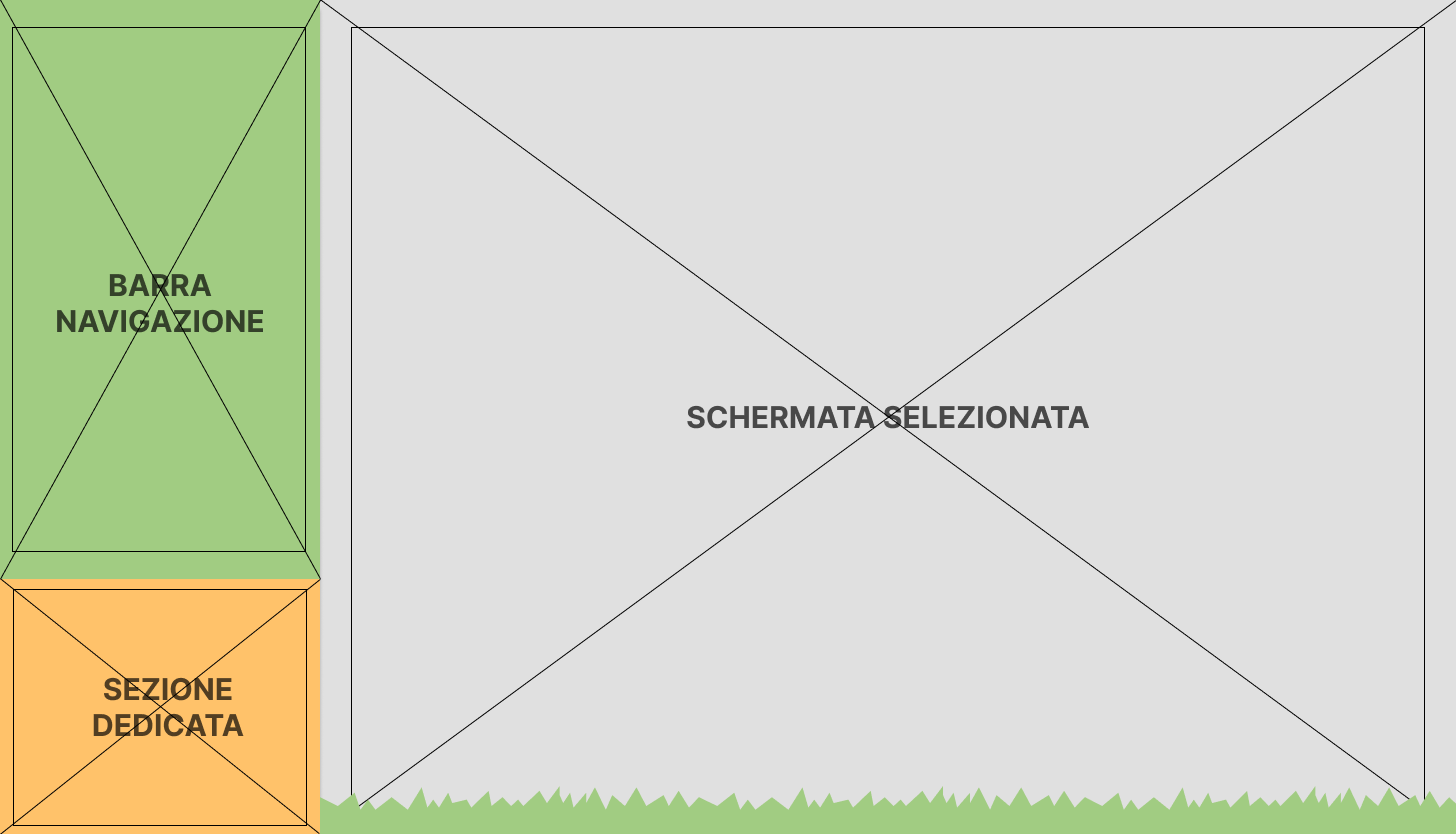
\includegraphics[width=0.7\textwidth]{img/mainStructure.png}
    \caption{Pulsante per mostrare e nascondere il codice QR identificativo del totem per la condivisione dei dati da APP}
    \label{fig:viewStruct}
\end{figure}

\subsection{Scansione codice QR totem}
In fondo alla barra di navigazione verticale si è posizionato il codice QR che identifica il totem per la condivisione dei progressi dell'utente tramite app.
In figura \ref{fig:depositIconsQR} viene mostrata l'icona del pulsante. Si compone di due immagini: un vaso ed una freccia verde (figura \ref{fig:hideQR}). Al tocco del pulsante la freccia svanisce, il vaso si ingrandisce fino a contenere al suo interno il codice QR (figura \ref{fig:showQR}).

\begin{figure} [h]
    \centering
    \subfloat[Codice QR del totem nascosto]{
        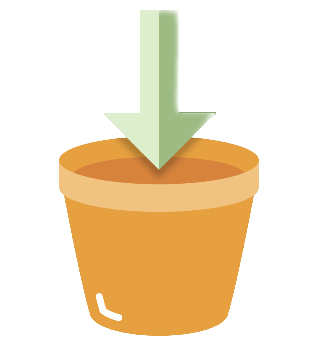
\includegraphics[width=4cm]{img/depositIcon.png}
        \label{fig:hideQR}
    }
    \vspace{1cm}
    \subfloat[Codice QR del totem visibile]{
        
\includegraphics[width=4cm]{img/depositQR.png}
        \label{fig:showQR}
    }
    \caption{Pulsante per mostrare e nascondere il codice QR identificativo del totem per la condivisione dei dati da APP}
    \label{fig:depositIconsQR}
\end{figure}
%
\subsection{Homepage}
Per la \textit{homepage} sono stati pensati due design alternativi: uno mette in risalto gli utenti mentre l'altro fornisce una visione più globale della partecipazione degli utenti.
Il primo è organizzato in mensole su cui poggiano i vasi contenenti l'alberello che rappresenta il livello dell'utente (figura \ref{fig:shelfHome}). Più alto è il livello raggiunto più rigogliosa e prospera sarà la chioma. Le mensole sono disposte in modo da occupare lo spazio a disposizione. Questa soluzione riduce molto la quantità di utenti visualizzabili per volta, costringendo ad una paginazione delle mensole navigabile con frecce o pulsanti per cambiare pagina (questo dettaglio nel mockup non è stato inserito).
La seconda alternativa di \textit{homepage} invece permette di visualizzare molti più elementi rispetto alla precedente. La visualizzazione cambia prospettiva, viene abbandonata l'idea delle mensole e vengono mostrate le chiome degli alberi in visione aerea come se si guardasse un bosco dall'alto(figura \ref{fig:forestHome}).

\begin{figure} [h]
    \centering
    \subfloat[Visualizzazione a mensole]{
        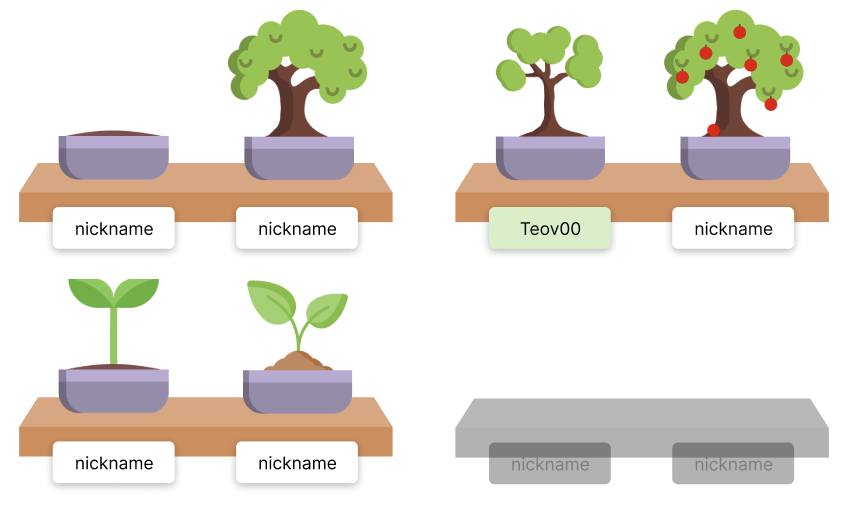
\includegraphics[width=0.45\textwidth]{img/shelfViewHome.png}
        \label{fig:shelfHome}
    }
    \subfloat[Visualizzazione a bosco]{
        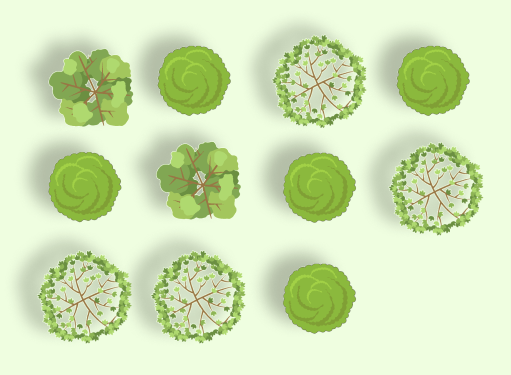
\includegraphics[width=0.45\textwidth]{img/forestViewHome.png}
        \label{fig:forestHome}
    }
    \caption{Possibili design di visualizzazione degli elementi della \textit{homepage}}
    \label{fig:homepages}
\end{figure}

In entrambe le alternative è presente un pannello che scende dall'alto che mostra i progressi condivisi dell'utente relativi all'elemento selezionato.

\subsubsection{Pannello dettagli utente}
Di questo componente sono stati pensati tre diverse possibili soluzioni: i primi due si assomigliano se non per qualche dettaglio come la mensola anziché del cordino in basso (figure \ref{fig:shelfDetail} e \ref{fig:cordDetail}) mentre l'ultimo si discosta completamente (figura \ref{fig:rectDetail}) sia graficamente sia per animazione.
\begin{figure} [h]
    \centering
    \subfloat[Stile mensola]{
        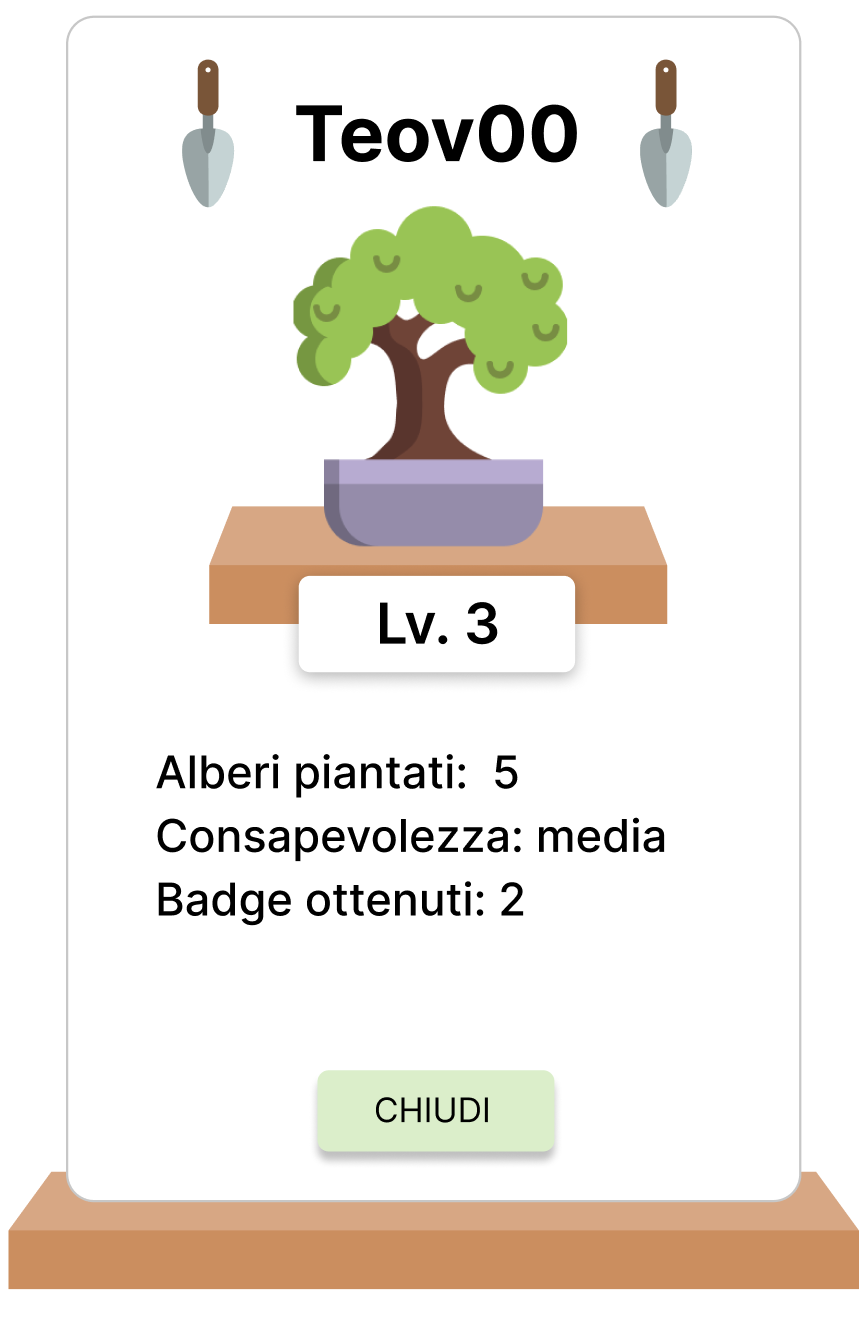
\includegraphics[width=0.33\textwidth]{img/shelfDetail.png}
        \label{fig:shelfDetail}
    }
    \subfloat[Stile tendina]{
        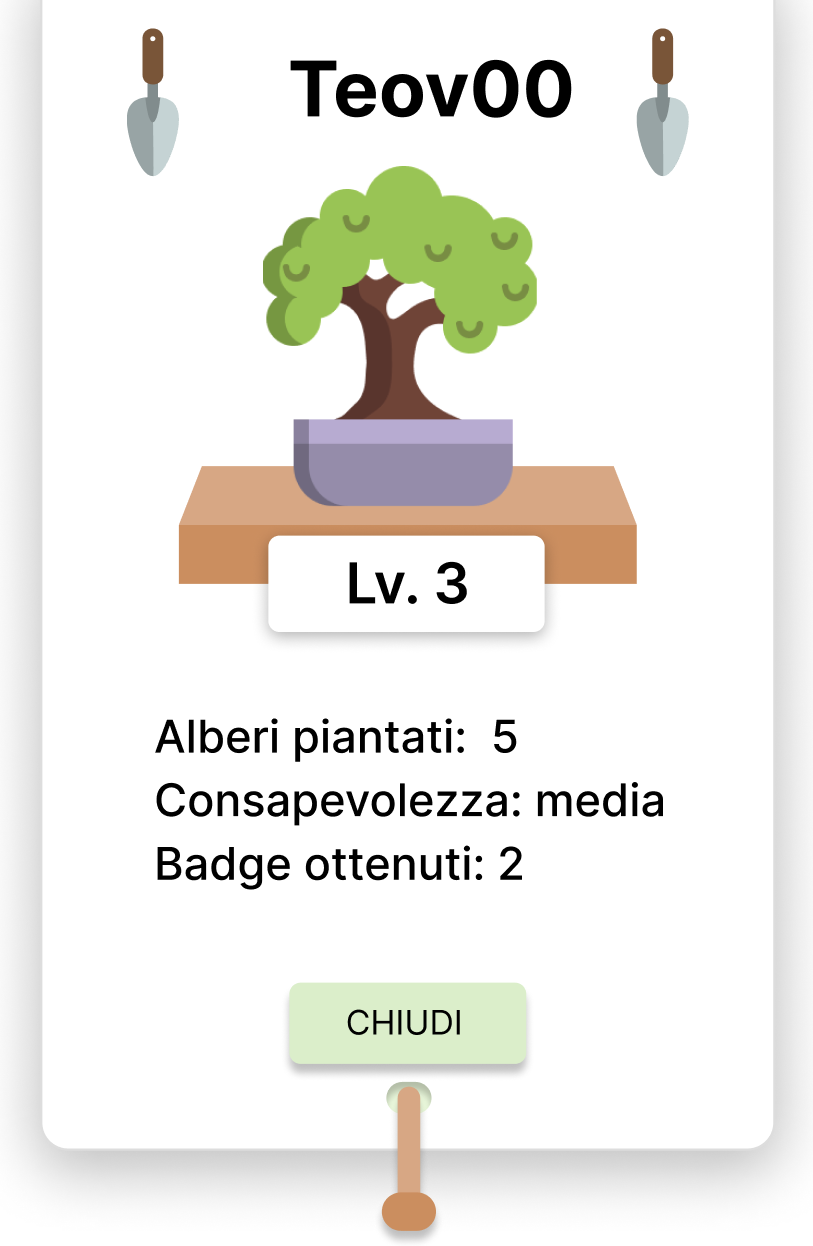
\includegraphics[width=0.33\textwidth]{img/cordDetail.png}
        \label{fig:cordDetail}
    }
    \subfloat[Stile rettangolo]{
        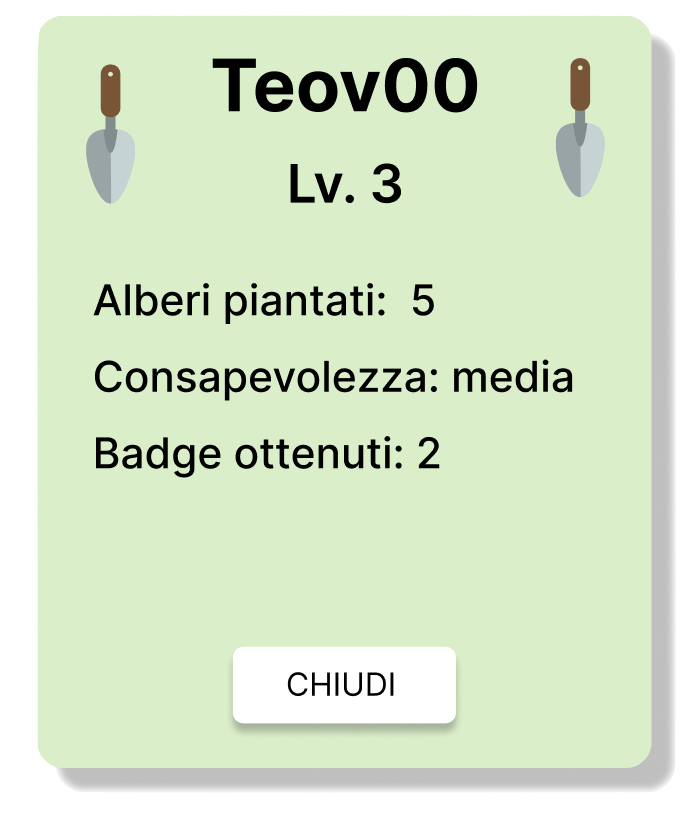
\includegraphics[width=0.33\textwidth]{img/rectDetail.png}
        \label{fig:rectDetail}
    }
    \caption{Tre diversi stili per il pannello dei dettagli: mensola, tendina e rettangolo}
    \label{fig:detailBanner}
\end{figure}
%
\subsection{Pagina statistiche}
La pagina delle statistiche presenta una griglia di sei elementi, che chiameremo contatori, uno per ogni dato statistico (\ref{fig:statsPage}). Al tocco di un contatore questo si trasforma diventando quadrato e mostrando una breve descrizione del dato statistico (\ref{fig:descrShowedStats}).

\begin{figure} [h]
    \centering
    \subfloat[]{
        
\includegraphics[width=0.3\textwidth]{img/plantedTreeStats.png}
        \label{fig:iconStats}
    }
    \subfloat[]{
        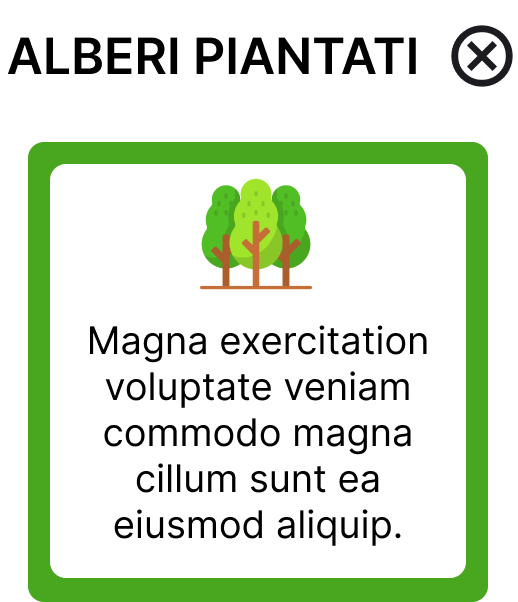
\includegraphics[width=0.3\textwidth]{img/plantedTreeStatsdescr.png}
        \label{fig:descrShowedStats}
    }
    \caption{Esempio di contatore nella pagina delle statistiche}
    \label{fig:statCircle}
\end{figure}

\begin{figure}
    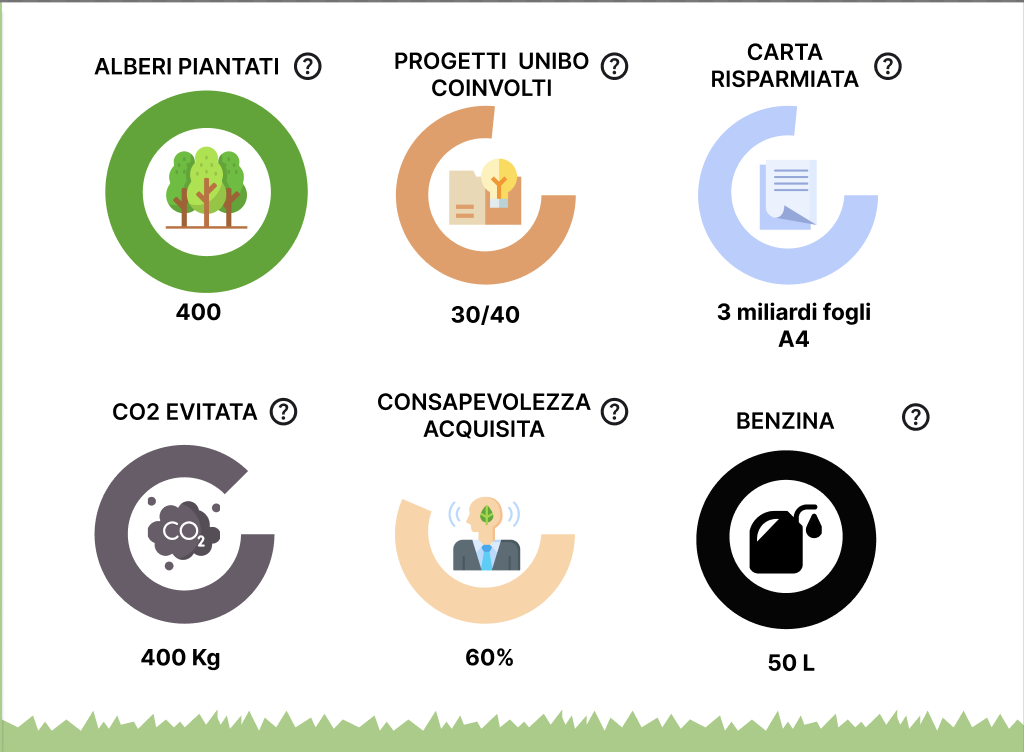
\includegraphics[width=0.8\textwidth]{img/statsPage.png}
    \caption{Mockup della schermata delle statistiche}
    \label{fig:statsPage}
\end{figure}
%
%
\subsection{Pagina della classifica}

%
\subsection{Pagina delle informazioni}
Inizialmente pensata come una unica pagina scorribile, simile ad una pagina web, ma poteva risultare difficile scorrere il dito su un monitor pubblico e più indicato per interazioni come tocchi invece di strisciamenti con forti attriti.
Si è optato per un design semplice a griglia di \enquote*{piastrelle} (\textit{tiles}), dove a colpo d'occhio è possibile avere le informazioni principali e per maggiori dettagli basta toccare la \textit{tile} interessata.

\begin{figure} [h]
    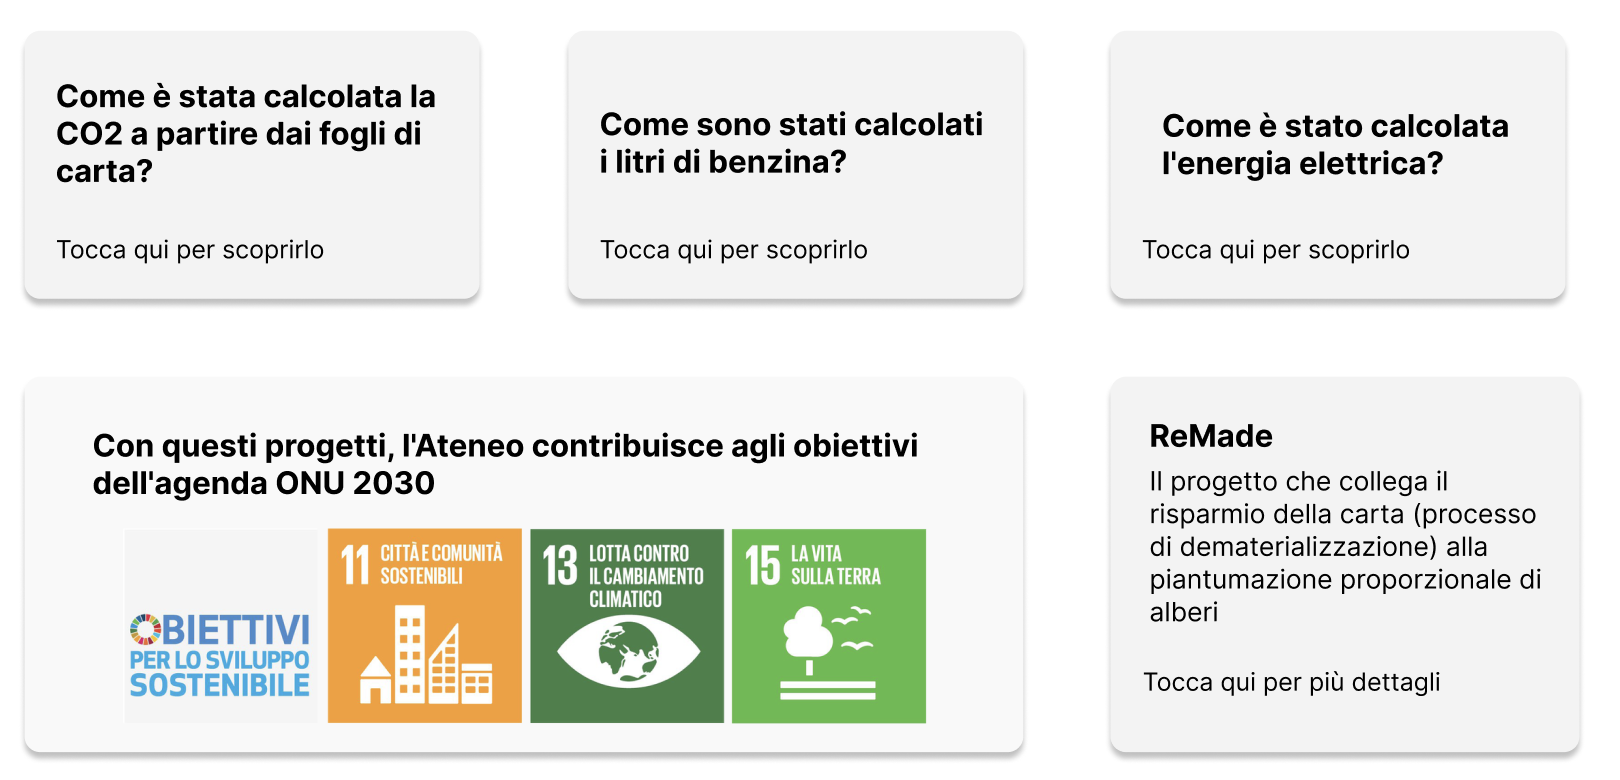
\includegraphics[width=0.8\textwidth]{img/infoPage.png}
    \caption{\textit{Mockup} della schermata delle informazioni}
    \label{fig:infoPage}
\end{figure}

%
%
%
\section{Tecnologie impiegate}
Disclaimer dove dico che per entrambe le piattaforme, applicazione mobile e totem interattivo, sono state utilizzate le medesime tecnologie nella progettazione e sviluppo.

\subsection{Figma}
%
\subsection{Visual Studio Code}
%
\subsection{Git}
Version Control System VCS
%
\subsection{Flutter}
%
\subsection{Firebase Realtime}
%
\subsection{Codici QR}
%
% \subsection{Applicazione Mobile}
% \subsection{Pagina Web Totem}